\documentclass[12pt]{article}

\usepackage[T1]{fontenc}
\usepackage[utf8]{inputenc}

\usepackage[frenchb]{babel}
\usepackage{amsmath}
\usepackage{amssymb}
\usepackage{amsfonts}
\usepackage{color}
\usepackage{caption}
\usepackage{easytable}
\usepackage{epsfig}
\usepackage{etex}
\usepackage{etoolbox}
\usepackage{here}
\usepackage{layout} % \layout au début de doc -> longueurs caractéristiques de la mise en page
\usepackage{makeidx}
\usepackage{mathrsfs}
\usepackage{mathtools}
%\usepackage{nopageno}
\usepackage{pslatex}
\usepackage{pstricks}
\usepackage{pstricks-add}
%\usepackage[retainorgcmds]{IEEEtrantools} % des beaux tableaux (équations, matrice etc...) cf rapport TIPE
\usepackage{wrapfig}
\usepackage{lmodern}
\usepackage{eurosym}
\usepackage{csvsimple}
\usepackage{booktabs}
\usepackage{longtable}
\usepackage[french]{varioref}
\usepackage{listings}
\usepackage{epstopdf}

\usepackage{tikz}
\usetikzlibrary{shapes.geometric}
\usetikzlibrary{arrows}

\usepackage{float}
\usepackage{pgfplots}
\usepackage[version=3]{mhchem}
\usepackage{siunitx}
\sisetup{
unitsep = \cdot,
decimalsymbol = comma,
expproduct = \cdot
}

\usepackage[coverpage,fancysections,twoside]{polytechnique-psc}


\usepackage{url}
\usepackage{breakurl}
\def\UrlBreaks{\do\/\do-\do_}
\usepackage[breaklinks]{hyperref}
\hypersetup{%
 pdftitle = {PSC - Rapport final},%
 pdfsubject = {},%
 pdfkeywords = {},%
 pdfcreator = {pdfLaTeX},%
 pdfproducer = {pdfLaTeX},%
 bookmarksnumbered = true,%
 pdfstartview = FitH,%
 pdfpagelayout = OneColumn,%
 colorlinks = false,%
 pdfborder = {0 0 0}%
}

\newcommand{\smartgrid}{\emph{Smart-Grid}}
\newcommand{\smartgrids}{\emph{Smart-Grids}}
\newcommand{\D}{\mathrm{d}}
\renewcommand{\thefootnote}{(\roman{footnote})}

%\titleformat{\chapter}[hang]{\Huge\bfseries\sffamily}{\LARGE}{0em}{}[]

\title{Rapport final}
\subtitle{Modélisation de l'impact de la recharge des véhicules électriques sur le réseau}
\author{ Vincent \textsc{Dufour-Décieux} \\ Odilon \textsc{Formery} \\ Ahmed \textsc{Krarti} \\ Louis \textsc{Legrand} \\ Augustin \textsc{Lenormand} \\ Camille \textsc{Masset} }

\begin{document}

\maketitle

\newpage
\renewcommand{\thepage}{}
\thispagestyle{empty}
\null
\newpage

\renewcommand{\thepage}{\arabic{page}}
\setcounter{page}{1}

\section*{Introduction}
\addcontentsline{toc}{section}{Introduction}

Nos habitudes de consommation d'énergie sont appelées à évoluer grandement dans les années à venir.
En effet la prise de conscience écologique, la fluctuation des cours du pétrole et la baisse du coût des technologies durables doivent nous amener à transformer notre comportement. 
Par exemple dans le domaine du transport, de nombreuses études sont menées depuis une vingtaine d'années pour trouver un remplaçant aux énergies fossiles, tel que les biocarburants ou les moteurs à hydrogène.
Au vu de l'orientation actuelle prise par les constructeurs il apparait que le véhicule électrique est le meilleur concurrent des véhicules thermiques. 
Afin d'anticiper cette profonde évolution du marché de l'énergie il faut prévoir l'impact qu'aura ce changement de demande énergétique du pétrole vers l'électricité. 

Faisons une expérience de pensée: supposons que les 38~millions de véhicules actuellement en France soient tous des véhicules électriques. Si toutes ces voitures se rechargent en même temps, en demandant une puissance de \SI{3.5}{\kilo\watt}, cela nécessite de produire une puissance totale de \SI{133}{\giga\watt}. Sachant qu'une centrale nucléaire ne délivre qu'une puissance d'un gigawatt, il faudra trouver d'autres solutions pour répondre au problème. C'est pour cela qu'il faut prévoir et modéliser l'impact qu'aura la recharge des véhicules électriques sur le réseau. Cela nécessite non seulement de prévoir le nombre de véhicules électriques qui seront en circulation dans vingt ans, mais aussi de modéliser le comportement des utilisateurs de véhicules électriques. 

En outre, on peut déjà supposer que cette recharge s'effectuera à partir de l'heure de retour du travail, entre 18~heures et 20~heures. Or c'est déjà l'heure du pic de consommation en France. Les fournisseurs d'énergie doivent donc augmenter la flexibilité de l'offre énergétique afin de s'adapter à cette nouvelle demande. Une des solutions peut être d'utiliser les batteries des véhicules électriques comme des \og{}mini-centrales\fg{}, capables lorsqu'elles sont branchées de fournir de l'énergie au réseau lorsque celui-ci en demande plus. On se place donc ici dans une problématique de \smartgrid{} (réseau intelligent) et d'agrégateurs de flexibilité. 

L'objectif de ce PSC est d'évaluer l'impact qu'aura la recharge des véhicules électriques sur le réseau dans quinze ans, et de voir quelles sont les solutions qui peuvent être utilisées dans le cadre du \smartgrid{}. Pour cela nous avons mené une étude sur le comportement des utilisateurs de véhicules, afin de connaitre leurs habitudes de recharge et de consommation, puis nous avons cherché à modéliser la diffusion des véhicules électriques en France afin d'avoir une idée de la taille du parc automobile en 2025. Enfin nous avons produit un programme informatique permettant de mettre en place le modèle et d'en obtenir des données sur la puissance demandée par la recharge des véhicules électriques.

\section{Évolution du projet}
	Notre projet était au départ d'étudier l'usure des batteries d'appareils électriques, tels que les téléphones portables, au cours de leurs cycles de charge et décharge. Nous avons ensuite pris contact avec l'entreprise GDF-Suez qui proposait de faire un PSC sur \og{}L'étude d'un algorithme de charge/décharge des véhicules électriques\fg{}. Cependant GDF-Suez nous a appris que le projet avait déjà été fait et nous a proposé un autre projet basé cette fois-ci sur une étude plus orientée sur le comportement des utilisateurs de véhicules électriques. C'est ainsi que nous avons entamé ce PSC sur la modélisation de l'impact de la recharge des véhicules électriques sur le réseau. 
	
	Notre planning prévisionnel était de faire de la recherche de données sur le comportement des utilisateurs et sur les caractéristiques des véhicules électriques jusqu'à fin décembre. Ensuite nous devions entamer la partie modélisation et implémentation du code.
	
	Concrètement le planning prévisionnel a été bien tenu. La recherche de données et l'exploitation de ces données nous a demandé beaucoup de travail au début du PSC. En effet comme le véhicule électrique est encore un marché de niche, il existe très peu d'études sur le comportement de leurs utilisateurs. Nous avons donc prospecté quelques études faites sur des petits échantillons et nous avons extrapolées des données sur les utilisateurs de véhicules thermiques, en considérant que leurs comportements varient peu avec les utilisateurs de véhicules électriques (pour les horaires de départ et de retour du travail et les distances parcourues par exemple).
	
	Parallèlement à cette recherche documentaire nous nous sommes penchés sur la forme qu'aura le résultat produit par notre modèle. Nous avons donc opté pour une courbe de la puissance consommée par la recharge des véhicules électriques en fonction de l'heure de la journée. 
	Nous avons commencé la partie modélisation au mois de janvier. Nous pensions pouvoir la terminer plus rapidement, mais en réalité nous avons rencontré des difficultés nouvelles. En effet il y avait de nombreux paramètres qui dépendaient les uns des autres, et produire un modèle mathématique pour définir ces interactions n'était pas évident.
	Nous avons produit un premier programme informatique basique pour le rapport intermédiaire. Celui-ci nous a permis de tester rapidement notre modèle, mais était limité dans les modifications que l'on pouvait lui apporter, notamment au niveau du \smartgrid{} ou du comportement des utilisateurs.
	Nous nous sommes alors lancés dans une partie purement algorithmique, afin de produire un programme qui soit rapide à exécuter pour de nombreux véhicules et facilement modifiable. Le travail en groupe était plus difficile à mettre en place lors de ce moment car nous ne possédions pas tous les connaissances requises en informatique.
	
	C'est pour cela qu'une partie du groupe s'est penché sur une nouvelle problématique apportée par le PSC : la prévision du nombre de véhicules électriques dans une quinzaines d'années. Ce n'était pas une partie que nous avions mis dans notre planning de départ mais elle nous permet d'apporter des éléments concrets pour les données d'entrée de notre modèle.
	

\section{Contexte et données}

\subsection{Enjeux et problématique}

Dans cette partie nous étudierons les pics de consommations et les solutions proposées par GDF-Suez pour pouvoir les effacer. Afin de mieux comprendre ces pics nous commencerons par les replacer dans le contexte plus global de la distribution de l'électricité en France. Nous détaillerons ensuite les origines et manifestations des pics de consommations. Enfin nous expliquerons les concepts de \smartgrid{} et d'agrégateurs de flexibilité, qui sont respectivement un nouveau type de réseau électrique et un nouvel acteur du marché de l'électricité.


\subsubsection{Production et distribution de l'électricité}

Le prix de l'électricité, celui que les français peuvent lire sur leur facture, est composé de quatre parties (chiffres moyens en 2013) \cite{coutElec}:
\begin{itemize}
	\item la production (\SI{31}{\percent});
	\item l'acheminement par le gestionnaire de réseau (\SI{30}{\percent});
	\item la commercialisation par le fournisseur (\SI{8}{\percent});
	\item les taxes et la contribution au service public de l'électricité (\SI{31}{\percent}).
\end{itemize}

\bigskip

Précisons ce qui se cache derrière ces parties.
La production est l'étape de transformation des sources d'énergie en électricité.
En France, la principale source d'énergie est le nucléaire (\SI{78}{\percent}); viennent ensuite les sources thermiques (charbon, gaz) et hydrauliques (\SI{9}{\percent} chacune), puis les énergies renouvelables intermittentes (éolien: \SI{2}{\percent}, photovoltaïque: \SI{1}{\percent}) ou continue (géothermie: \SI{1}{\percent}).

Le nucléaire, l'hydraulique et la géothermie permettent une production continue (avec des ajustements possibles pour les barrages hydroélectriques), et constituent donc une base solide pour la production électrique en France. Les sources thermiques sont essentiellement utilisées en période de forte consommation, car il est très rapide de mettre en fonctionnement une centrale à charbon par exemple, mais de telles centrales sont très polluantes (rejet de gaz à effet de serre dans l'atmosphère). Les autres sources d'énergie produisent en fonction des conditions climatiques (soleil, vent) et sont donc moins fiables. En particulier, on ne peut pas s'appuyer sur de telles sources d'énergies pour faire face à un pic de consommation.

L'acheminement consiste à amener l'électricité depuis la centrale de production vers le consommateur final. On peut décomposer cet acheminement en deux parties : le transport (lignes à haute et très haute tension) et la distribution (lignes à moyenne et basse tension). Les gestionnaires de réseaux d'électricité sont chargés de l'entretien et du bon fonctionnement des réseaux (sécurité, dépannage, qualité, relevé des compteurs). Ils sont rémunérés par le Tarif d'Utilisation des Réseaux Publics d'Électricité (TURPE), fixé par l'État. Les gestionnaires de réseaux sont RTE pour le transport et ERDF et les ELD (Entreprises Locales de Distribution) pour la distribution.

La commercialisation est assurée par le fournisseur qui est le contact privilégié du client. Il est aussi en relation avec les gestionnaires de réseaux de distributions. Il répercute les prix de l'acheminement et les taxes dans ses tarifs. Le consommateur peut choisir entre des prix réglementés fixés par les pouvoirs publics et proposés par les distributeurs historiques (comme EDF) ou une offre à prix de marché (contrat).

L'électricité est soumise à quatre taxes fixées par les pouvoirs publics : la TVA, la Contribution au Service Public de l'Électricité (CSPE), la Taxe sur la Consommation Finale d'Électricité (TCFE) et la Contribution Tarifaire d'Acheminement (CTA). La CSPE permet essentiellement d'investir dans le développement des énergies renouvelables et de financer le surcoût de la production d'électricité dans les zones non connectées au réseau continental. La TCFE est perçue par les communes et les départements et permet de financer les travaux sur les installations électriques locales. La CTA finance partiellement les retraites des salariés des gestionnaires de transport.
Les fournisseurs rencontrent des difficultés à répondre à la demande des clients pendant certaines périodes : les pics de consommation.


	\subsubsection{Pic de consommation}
	Une pointe de consommation électrique est la consommation la plus élevée sur un réseau électrique. Elle peut résulter de plusieurs facteurs tels que l'heure de la journée ou la température extérieure, ainsi que le montre la figure~\vref{courbeCharge}.
	
	On en distingue trois types majeurs :
	\begin{itemize}
		\item les pointes journalières qui se produisent souvent en fin de journée un jour de semaine, lorsque les personnes rentrent du travail; la pointe sera plus accentuée dans les réseaux où le chauffage de l'eau et les appareils électroménagers utilisent l'électricité plutôt que le gaz;
		\item les pointes saisonnières peuvent survenir en été ou en hiver (cas de la France), mais dans les deux cas, les températures extrêmes influent sur la demande de climatisation ou de chauffage électrique des ménages;
		\item certaines pointes sont aussi causées par les infrastructures d'utilités publiques telles que l'éclairage public ou le transport ferroviaire.
	\end{itemize}

\bigskip

On observe en France que la pointe progresse plus vite que la consommation électrique : elle augmente de \SI{3}{\percent}, alors que, dans le même temps, la consommation électrique connait une hausse de \SI{0.6}{\percent}. Plusieurs raisons en sont à l'origine, notamment la place du chauffage électrique et le développement de nouveaux usages de l'électricité (équipements électroménagers et informatiques, recharges multiples). Il est donc nécessaire d'agir rapidement pour lutter contre ces pics de consommation qui coutent cher et ont un impact environnemental au travers des augmentations d'émission de \ce{CO2}.
Par exemple, la perte d'un degré de température se traduit en France en 2012 par une augmentation estimée d'électricité de \SI{2300}{\mega\watt} contre \SI{600}{\mega\watt} en Grande-Bretagne \cite{picFrance}.

Quelles sont les solutions pour gérer ces pics ? Plusieurs moyens sont mis en \oe{}uvre par les gestionnaires de réseau.
La solution la plus évidente et la plus ancienne consistait en l'augmentation de la capacité de production par le biais de construction de nouvelles infrastructures de production, de transport et de distribution. Mais cette solution a très vite atteint ses limites d'une part car elle présente des risques environnementaux (émission de \ce{CO2}) mais aussi des risques de \emph{blackout} dus à la surcharge d'alimentation.
Une autre solution consiste à baisser le niveau de la consommation en commandant à un opérateur dit \og{}d'effacement\fg{} la coupure immédiate et coordonnée de certains postes de consommation; tout cela est géré par des réseaux intelligents : les \smartgrids{}.

\bigskip

\begin{figure}[!h]
	\centering
	\begin{tikzpicture}
	\begin{axis}[
	legend entries = {21/01/2015, 17/07/2014},
	legend style = {at = {(0.95, 0.05)}, anchor = south east}, 
	/pgf/number format/.cd,
	use comma,
	1000 sep={ },
	height = 8cm,
	width = 15cm,
	axis x line = bottom,
	ymin = 0,
	axis y line = left,
	xlabel = Heures,
	ylabel = Consommation (MW)
	]
	\addplot[mark = , smooth, color=blue] table[x=Heures,y=2015-01-21] {fig/courbesRTE.txt};
	%					\addlegendentry{21/01/2015};
	\addplot[mark =, smooth, color=red] table[x=Heures,y=2014-07-17] {fig/courbesRTE.txt};
	%					\addlegendentry{17/07/2014}
	\end{axis}
	\end{tikzpicture}
	\caption{Courbe de charge du réseau français un jour d'hiver (en bleu) et un jour d'été (en rouge)}
	\label{courbeCharge}
\end{figure}


\subsubsection{Les \smartgrids{}}

L'effacement résidentiel consiste à réduire temporairement la consommation d'électricité d'un grand nombre de petits sites, en particulier de logements, de façon à diminuer la demande \cite{effResidentiel}. Il s'agit par exemple d'interrompre brièvement, mais de façon synchronisée, l'alimentation de radiateurs ou climatiseurs situés dans des logements pour, au total, réduire la consommation d'électricité d'une région ou du pays.

Les utilisateurs qui souscrivent à ce type de service se verront installé un boîtier dans le tableau électrique de leurs maisons. Le principal avantage de ce boîtier est qu’il permet de collecter les données des utilisateurs mais aussi de commander à distance certaines tâches (arrêt du chauffage, de la climatisation).Toutes ces tâches sont réalisées par un automate programmable qui concilie au mieux entre les exigences du gestionnaire du réseau et celles de l'utilisateur.

Avec le développement des nouvelles technologies de l'information et de la communication (TIC), les distributeurs (EDF, RTE, ERDF) ont pu moderniser leurs réseaux. Ces réseaux intelligents, autrement appelés \smartgrids{} permettent de tenir compte de la variabilité des sources de production d'électricité renouvelable, (à cause de leur dépendance vis-à-vis de la météo notamment), ainsi que de l'augmentation de la production dite décentralisée (parc éolien raccordé au réseau de distribution ou consommateur final disposant de panneaux photovoltaïques sur le toit de son habitat qui devient producteur d'énergie) et les ambitions de réduction des consommations d'énergie complexifient la gestion de l'équilibre entre production et consommation. En favorisant l'intégration des productions d'électricité à partir d'énergies de sources renouvelables, les \smartgrids{} ont un impact fort sur la réduction d'émission de \ce{CO2}.


Les effets de ces \smartgrids{} peuvent être développés grâce à un agrégateur de flexibilité que nous allons maintenant présenter.


\subsubsection{L'agrégateur de flexibilité}

L'agrégateur \cite{agregateur} est une prestation complémentaire, un intermédiaire entre le système électrique et ses utilisateurs. Il crée de la valeur pour ses clients en revendant de la flexibilité au système électrique, ce que l'on qualifie parfois de \og{}centrale électrique virtuelle\fg{}. Pour que tout cela fonctionne, il faut stocker de l'énergie pendant les périodes creuses pour pouvoir faire face aux pics. Ce stockage se fait au niveau:
\begin{itemize}
	\item individuel : grâce aux batteries des VE, aux ballons d'eau chaude;
	\item des bâtiments : inertie thermique, batterie chaude ou froide;
	\item des collectivités : barrage électrique, château d'eau;
	\item industriel : stockage de produits intermédiaires (cimenterie).
\end{itemize}
\bigskip

Cela nécessite:
\begin{itemize}
	\item de rendre les immeubles et les sites industriels qu'il pilote \og{}intelligents\fg{};
	\item de penser des modèles pour prévoir les résultats de son action;
	\item de recueillir des informations pour anticiper les évolutions du marché.
\end{itemize}
\bigskip

Malheureusement tout cela est assez lent à mettre en place pour plusieurs raisons : la loi NOME ne permet pas la mise en place de ces réseaux avant 2016 \cite{loiNome}, de plus le consommateur doit avoir la possibilité de revenir en mode \og{}normal\fg{} à tout moment, des études sur le comportement des utilisateurs doivent être faites pour pouvoir choisir les moments où effacer l'électricité ou non.

\subsubsection{Notre PSC et son inscription dans ce contexte}

Des solutions au problème des pics de consommation ont été apportées à travers les \smartgrids{} et l'agrégateur de flexibilité, cependant ces deux systèmes ont besoin d'informations sur la consommation d'électricité des clients pour soit effacer la consommation à travers les \smartgrids{}, soit pour savoir quand l'agrégateur devra redistribuer l'énergie accumulée. Les fournisseurs, tels que GDF Suez, peuvent obtenir cela pour les habitudes actuelles car la consommation d'électricité vient principalement de l'électroménager, de la lumière et du chauffage. Mais un changement commence à s'opérer dans le quotidien des individus et il s'agit de la voiture électrique. En effet, celle-ci va amener des consommations supplémentaires d'électricité à travers sa recharge et prévoir comment cela va influer sur les pics de consommation mérite une étude poussée. C'est là qu'intervient notre PSC : nous avons étudié le comportement des utilisateurs de véhicules électriques pour savoir quand ils rechargeront leur véhicule et quel effet cela aura sur le réseau. GDF Suez souhaite aussi gérer intelligemment l'augmentation des pics de consommation due aux véhicules électriques en apportant une nouvelle idée : lorsque le véhicule sera branché, il sera possible de ne pas le recharger pour repousser l'utilisation d'énergie à un moment où le réseau sera moins soumis à la demande ou même de fournir de l'énergie au réseau pour que l'effet bénéfique soit amplifié. Nous tenterons de prévoir le nombre de personnes intéressés par cette offre et comment elle influera sur le réseau au cours de notre étude.



\subsection{Données collectées}

Nous avons donc cherché des informations sur le comportement des utilisateurs de véhicules électriques que nous analyserons ensuite. Malheureusement, puisque leur nombre est aujourd'hui peu conséquent (environ \num{30000}) il est difficile de trouver des études sur ce sujet. Nous avons cependant réussi à en réunir quelques-unes:
\begin{itemize}
	\item une étude du Club Alsace Voiture \'Electrique \cite{clubalsace} sur les habitudes de ces utilisateurs. L'enquête nous donne des informations (fréquence des recharges des voitures, lieu d'utilisation des bornes,~...) réalisées auprès de 500 utilisateurs ;
	\item un échange avec La Poste nous a permis de recueillir des informations sur l'utilisation de leur flotte de \num{5000} véhicules électriques ;
	\item un échange avec \textit{Autolib'} nous a permis d'avoir des informations générales sur ces véhicules qui représentent environ \num{3500} véhicules ;
	\item des données techniques sur les différentes marques principales de véhicules électriques (nombre, consommation, autonomie,~...).
\end{itemize}
\bigskip

Ces données nous ont été utiles mais nous ne pouvions pas déterminer à quelles heures les trajets étaient effectués, quelles distances ont été parcourues ou d'autres informations de ce type qui sont cruciales pour pouvoir modéliser la demande en électricité due aux véhicules électriques en fonction de l'heure de la journée. Malheureusement, nous n'avons pas réussi à trouver ces informations pour les véhicules électriques, nous avons donc décidé de considérer que les données des voitures à essence pouvaient être extrapolées aux véhicules électriques. Nous avons ensuite concentré notre étude sur les jours ouvrés et dans ce cas, les principaux trajets de la journée sont ceux entre le domicile et le travail. Nous avons donc trouvé les données suivantes:
\begin{itemize}
	\item l'enquête \og{}La circulation routière en Île-de-France en 2010\fg{} \cite{OMNIL} réalisée par l'OMNIL qui possède une partie intéressante dans laquelle on voit le trafic routier en Île-de-France en fonction de l'heure de la journée. Nous avons trouvé de plus l'exploitation de cette enquête qui permet d'avoir accès aux informations de manière plus synthétique;
	\item l'\og{}Enquête auprès des salariés d'Île-de-France sur les transports en commun domicile-travail\fg{} \cite{ORSTIF} nous a permis d'en savoir plus sur ces trajets ce qui nous a  été très utile pour la modélisation;
	\item l'\og{}Enquête nationale des transports et des déplacements réalisés en 2008\fg{} \cite{enqueteGouv} qui nous a permis d'avoir accès à la distance moyenne des trajets et à leur durée moyenne.
\end{itemize}
\bigskip
En ce qui concerne l'acceptation du décalage de la recharge et du système \emph{Vehicle to Grid} par les utilisateurs nous nous sommes basés sur un sondage fait à l'échelle européenne par le consortium \emph{Grid for Vehicles} \cite{reacUtilisateurs}.

Ces données sont suffisamment récentes pour être utilisées lors de notre modélisation.

\section{Diffusion du véhicule électrique}

	\subsection{Différents modèles de diffusion}
	
		Le modèle de diffusion de Bass sert avant tout à prévoir l'évolution de l'adoption d'un nouveau produit dans une population donnée. Ainsi, il décrit l'intégration des innovations technologiques dans la population. Notre objectif est ici de déterminer le nombre de véhicules électriques en circulation en 2025. Étant donné qu'il existe peu d'études sur le sujet, il est judicieux d'adopter un modèle type Bass pour mesurer l'évolution de ce marché dans les prochaines années.
		
		
		Selon la théorie de Bass, on peut classer les utilisateurs en grandes classes : les innovateurs, les \emph{early adopters}, les \emph{early majority}, les \emph{late majority} et les retardataires. Cette classification, illustrée par la figure \vref{fig.BassUtilisateurs}, se fait par l'intermédiaire de deux facteurs essentiels: l'hétérogénéité des agents sociaux (aversion au risque, milieu social), et la capacité intellectuelle de l'individu.
		
		\begin{figure}[!h]
			\centering
			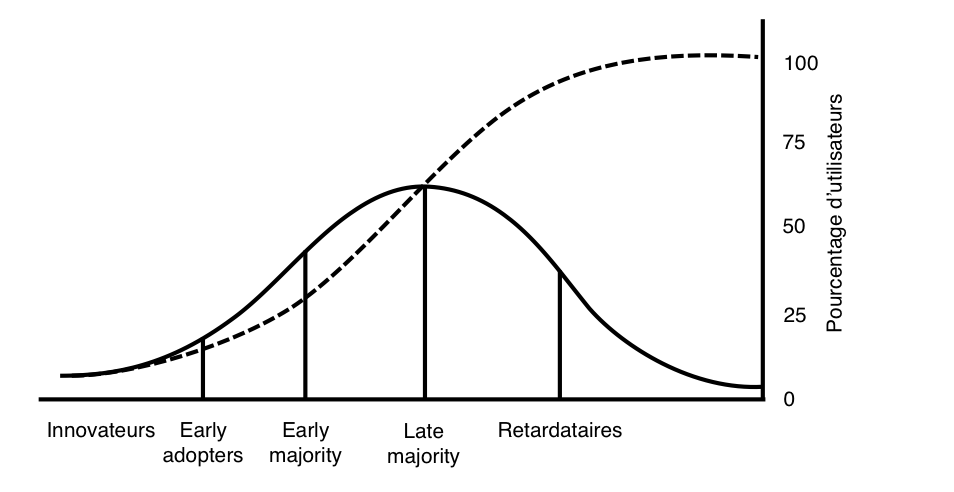
\includegraphics{fig/BassUtilisateurs.eps}
			\caption{Évolution du nombre d'utilisateurs d'une innovation technologique selon le modèle théorique de Bass. \label{fig.BassUtilisateurs}}
		\end{figure}
		
		Les modèles de diffusion peuvent être résumés dans une seule équation différentielle: 
		\[
			\dfrac{\D N(t)}{\D t} = g(t)(m-N(t))
		\]
		où $N(t)$ est le nombre cumulé d'individus ayant adopté la technologie à la date $t$, $m$ est le seuil maximal du nombre d'acheteurs potentiels, c'est-à-dire la taille du marché, et $g(t)$ le \emph{coefficient de diffusion}.
		
		En fonction de la valeur du coefficient de diffusion $g(t)$, on trouve 3 modèles essentiels :
		\begin{enumerate}
			\item modèle des influences externes: $g(t) = p = \text{cste}$.
			Dans ce modèle, le paramètre $p$ peut être interprété comme l'ensemble des facteurs extérieurs qui agissent sur la prise de décision du consommateur (pouvoir des médias et des réseaux sociaux, par exemple);
			\item modèle des influences internes: $g(t) = q N(t)$ où $q$ est le \emph{coefficient d'imitation}. Dans ce modèle, le paramètre $q$ représente l'interaction entre les acheteurs potentiels et ceux qui ont déjà adopté la technologie, car pour un futur acheteur l'avis des autres consommateurs est primordial;
			\item modèle de Bass : $g(t) = p + q \frac{N(t)}{m}$. C'est un mélange des deux modèles précédents. Ainsi, sur un intervalle de temps $\Delta t$, le nombre d'individus qui adoptent la technologie est régi par deux phénomènes: 
			\begin{itemize}
				\item contagion, fonction du nombre d'individus ayant déjà adopté l'innovation (terme $q N(t)(m - N(t))$);
				\item saturation du fait de la présence du palier $m$.
			\end{itemize}
			La solution à ce problème est:
				\[
					N(t) = \dfrac{m - \dfrac{p (m - N_0)}{p + q \frac{N_0}{m}} \mathrm{e}^{-(p+q)t}}{1 - \dfrac{\frac{q}{m} (m - N_0)}{p + q \frac{N_0}{m}} \mathrm{e}^{-(p+q)t}}
				\]
			avec $N_0 = N(t = 0)$.
		\end{enumerate}
		
		Mais tous les modèles précédents supposaient l'existence d'une taille de marché $m$ constante. Cependant, en général, ce n'est pas le cas: on peut considérer l'arrivée de nouveaux conducteurs, les voitures qui parviennent en fin de vie... C'est pour cette raison que l'on adoptera dans notre approche le modèle de Sharif et Ramannathan avec une taille de marché dépendante du temps : $m(t) = m_0 \mathrm{e}^{gt}$.
		
		
		La résolution mathématique de ce problème se présente sous cette forme :
		\begin{gather*}
			N(t) = m_0 \mathrm{e}^{gt} \dfrac{\dfrac{\Phi_1 - \Phi_2}{2} - \Phi_3 \dfrac{\Phi_1 + \Phi_2}{2} \mathrm{e}^{-\Phi_1 t}}{q + q \Phi_3 \mathrm{e}^{-\Phi_1 t}} \quad \text{où} \\
			\Phi_1 = \sqrt{(g+p-q)^2 + 4pq} \qquad \Phi_2 = g + p - q \qquad \Phi_3 = \dfrac{\frac{\Phi_1 - \Phi_2}{2} - q \frac{N_0}{m_0}}{\frac{\Phi_1 + \Phi_2}{2} + q \frac{N_0}{m_0}}, \; (0 < N_0 \leqslant m_0).
		\end{gather*}


	\subsection{Utilisation des modèles de diffusion pour le marché du véhicule électrique}

		L'implémentation des modèles précédents pour l'étude du marché des véhicules électriques nécessite la détermination des paramètres $p$, $q$, $N_0$ et $m$ (ou $m_0$ et $g$).

		Pour ce faire, nous utilisons comme données d'entrée le tableau \vref{tab.immatriculeConception} qui est issu de chiffres préfectoraux:
		
	
			
		\begin{table}[!h]
			\centering
			{\footnotesize
			\csvautotabular{fig/tableau1.csv}}
			\caption{Nombres mensuels d'immatriculations de véhicules électriques entre janvier 2011 et mars 2015. \label{tab.immatriculeConception}}
		\end{table}

		Nous nous intéressons dans un premier temps au modèle classique de Bass, dans lequel le paramètre $m$ ne dépend pas du temps.

		La grandeur $N_0$ se lit directement sur la première ligne du tableau de données: en effet, les immatriculations de voitures électriques sont extrêmement faibles avant janvier 2011 et le volume de ces véhicules peut être considéré comme négligeable. Nous prenons donc $N_0 = 100$.

		Les autres paramètres s'obtiennent par utilisation de la méthode OLS qui nous a paru la plus appropriée et la plus fidèle. Le tracé de $X(t) = N(t) - N(t-1)$ en fonction de $N(t-1)$ donne la courbe de la figure \vref{fig.courbeXt}.
		
		\begin{figure}[!h]
			\centering
			\begin{tikzpicture}
				\begin{axis}[ 
				/pgf/number format/.cd,
				use comma,
				1000 sep={ },
				height = 8cm,
				width = 15cm,
				axis x line = bottom,
				axis y line = left
 				]
				\addplot[mark = +, draw = blue, smooth] file{fig/courbeXt.txt};
				\addplot[color = red, domain = 0:30000] {-4.55*10^(-7)*x^2+0.0414*x+238.79};
				\end{axis}
			\end{tikzpicture}
			\caption{Tracé de $X(t)$ en fonction de $N(t-1)$.\label{fig.courbeXt}}
		\end{figure}
		
		Une courbe polynomiale de second degré $X(t) = \alpha_1 + \alpha_2 N(t-1) + \alpha_3 N(t-1)^2$ s'ajuste au graphique obtenu avec les valeurs suivantes (coefficient de corrélation $R^2 = \num{0.49}$):
		\begin{align*}
			\alpha_1 &= \num{238.79}\\
			\alpha_2 &= \num{0.04141}\\
			\alpha_3 &= \num{-4.55e-7}
		\end{align*}

		On obtient les paramètres suivants :
		\begin{align*}
			p &= \dfrac{-\alpha_2 + \sqrt{\alpha_2^2 - 4 \alpha_1 \alpha_3}}{2} = \num{0.0024743185}\\
			q &= \dfrac{\alpha_2 + \sqrt{\alpha_2^2 - 4 \alpha_1 \alpha_3}}{2} = \num{0.0438843185}\\
			m &= \dfrac{-\alpha_2 - \sqrt{\alpha_2^2 - 4 \alpha_1 \alpha_3}}{2 \alpha_3} = \num{96507}
		\end{align*}

		L'ordre de grandeur de $m$ parait cohérent, le nombre de véhicules électriques roulant en 2014 étant d'environ \num{30000}. Ceci nous permet d'obtenir le profil de diffusion de la figure \vref{fig.courbeBass1}, dont la limite est égale à $m = \num{96507}$.

		\begin{figure}[!h]
			\centering
				\begin{tikzpicture}
					\begin{axis}[
					height = 8cm,
					width = 15cm,
					axis x line = bottom,
					axis y line = left,
					xlabel = mois,
					ylabel = nombre d'utilisateurs cumulés
					]
					\addplot[mark = none, draw = blue, smooth] file{fig/courbeBass.txt};
					\end{axis} 
				\end{tikzpicture}
			\caption{Profil de diffusion selon le modèle de Bass.\label{fig.courbeBass1}}
		\end{figure}

		Ce modèle semble avoir une durée de validité assez faible, puisque le palier $X = m$ est obtenu avant 2025. Essayons donc d'implémenter le modèle plus réaliste de Sharif et Ramannathan, dans lequel la capacité globale du marché $m$ dépend du temps, selon une loi exponentielle: $m(t) = m_0 \mathrm{e}^{gt}$.
		Nous reprenons les mêmes coefficients d'innovation $p$ et d'imitation $q$ que précédemment. Il est également logique d'adopter $m_0 = \num{96507}$ puisque $m(t = 0) = m_0$.
		Reste enfin à trouver une valeur pour le coefficient $g$. N'ayant aucune méthode à notre disposition pour le déterminer, nous adoptons $g = 0,035$ \footnote{Valeur utilisée dans une étude sur la diffusion de l'accès à Internet, au sein de la population française (A. Kijek, T. Kijek, \textit{Operations research and decisions}, \textbf{2010}, 3-4, \textit{53-68}).}.
		Le graphe obtenu présenté en figure \vref{fig.SharifRaman}.
		
		\begin{figure}[!h]
			\centering
			\begin{tikzpicture}
				\begin{axis}[
				height = 8cm,
				width = 15cm,
				axis x line = bottom,
				axis y line = left,
				xlabel = mois,
				ylabel = nombre d'utilisateurs cumulés
				]
				\addplot[mark = none, draw = blue, smooth] file{fig/SharifRaman.txt};
				\end{axis}
			\end{tikzpicture}
			\caption{Profil de diffusion selon le modèle de Sharif et Ramannathan.\label{fig.SharifRaman}}
		\end{figure}
		
	\clearpage
		
	\subsection{Conclusion}
		
		Les résultats obtenus sont insuffisants. Le premier profil montre une saturation trop rapide, le marché étant supposé de taille fixe $m$: le point d'inflexion est atteint à $t^* = -\dfrac{1}{p+q} \log{\frac{p}{q}} = 62 \text{ mois}$.

		En ce qui concerne le deuxième modèle utilisé, le profil obtenu ne correspond pas aux données que nous avions initialement. Le graphe de la figure \vref{fig.diverSharifRam} présente la divergence entre la réalité (courbe en pointillés) et la théorie.
		
		\begin{figure}[!h]
			\centering
			\begin{tikzpicture}
				\begin{axis}[
				height = 8cm,
				width = 15cm,
				axis x line = bottom,
				axis y line = left,
				xlabel = mois,
				ylabel = nombre d'utilisateurs cumulés
				]
				\addplot[mark = none, draw = blue, smooth] file{fig/graphe5.txt};
				\addplot[mark =+, draw = red, only marks] file{fig/graphe4.txt};
				\end{axis}
			\end{tikzpicture}
			\caption{Divergence entre la réalité et la théorie de Sharif et Ramannathan \label{fig.diverSharifRam}}
		\end{figure}
		
		De plus, la taille n'est pas illimitée comme le laisserait supposer l'exponentielle $m(t)$ : en réalité, $m$ augmente par paliers, correspondant par exemple aux innovations technologiques... Le temps caractéristique $\tau$ est de 29 mois, ce qui donnerait un modèle valable jusqu'en 2020 environ.
		
		L'extrapolation du premier profil (figure \vref{fig.extraBass}) jusqu'en janvier 2025 nous permet de supposer un nombre d'utilisateurs de véhicules électriques de $N = \num{163000}$ environ. Nous conservons ce chiffre pour l'étude qui suivra.
		
		\begin{figure}[!h]
			\centering
			\begin{tikzpicture}
				\begin{axis}[
				height = 11cm,
				width = 15cm,
				axis x line = bottom,
				axis y line = left,
				xlabel = mois,
				ylabel = nombre d'utilisateurs cumulés
				]
				\addplot[mark = none, draw = blue, smooth] file{fig/courbeBass.txt};
				\addplot[mark=none, ycomb, color = red] plot coordinates{(169,169*1101-22438)};
				\addplot[color = red, domain = 22438/1101:169]{1101*x -22438};
				\end{axis}
				\end{tikzpicture}
			\caption{Extrapolation à partir du modèle de Bass \label{fig.extraBass}}
		\end{figure}

\lstset{ %
    language = c++, %
    basicstyle = \ttfamily%
}

\section{Modélisation numérique}
	\subsection{Motivations et objectifs}
		\subsubsection{Motivations}
			En parallèle de notre étude de la diffusion du véhicule électrique, nous avons travaillé sur le modèle permettant d'évaluer l'impact futur des véhicules électriques sur la consommation globale d'électricité. L'usage de l'outil informatique nous a semblé essentiel pour une telle modélisation, étant donné le nombre important de paramètres et la taille de nos échantillons de calculs. Nos efforts se sont donc tournés vers l'élaboration d'un algorithme de calcul capable de produire une courbe représentant la puissance nécessaire à la recharge d'un véhicule électrique au cours du temps.

			En répétant cet algorithme pour un nombre donné de véhicules, et en sommant les puissances calculées, on obtient ainsi une courbe de charge globale pour cette flotte de véhicules.

			Cette production visuelle nous a semblé la plus à même d'être exploitée dans le cadre de notre étude. Un excès de précision dans la production des résultats numériques n'aurait pas eu de sens, étant donné la nature statistique de nos données, et les différentes approximations et extrapolations effectuées.

		\subsubsection{Objectifs}
			
			Les objectifs principaux de notre travail de modélisation sont donc:
			\begin{enumerate}
				\item produire un résultat visuel et facilement exploitable de la charge imposée au réseau par une flotte de véhicules électriques, flotte la plus représentative possible de la réalité (modèle de véhicule, utilisation,~...);
				\item permettre de modifier aisément certains paramètres du modèle comme la taille de l'échantillon ou les hypothèses de flexibilité (\smartgrid{}, Vehicule to Grid);
				\item présenter un algorithme et un cheminement logique clair et détaillé, pour permettre une réutilisation ou une adaptation ultérieure aisée.
			\end{enumerate}
			Nous nous sommes donc rapidement attachés à développer une structure et un organigramme assez précis de l'algorithme. Ainsi même si des contingences techniques apparaissaient et retardaient notre production d'un programme fonctionnel, et donc de courbes résultats, notre travail pourrait tout de même être une base suffisamment claire et modulaire pour une exploitation future.

	\subsection{Cheminement de pensée}
		Après un premier algorithme naïf et peu exploitable, présenté dans le rapport intermédiaire, nous avons choisi d'aborder le problème différemment.
		
		Pour notre modèle final nous avons décidé de travailler avec une approche plus atomique. Nous avons en effet choisi de considérer les véhicules individuellement, et définis de manière indépendante ---~au lieu d'un véhicule moyen~---  et de faire évoluer chaque véhicule pendant la durée de la simulation selon ses caractéristiques propres.
		Cela nous a permis de définir nos véhicules avec une cohérence physique plus grande que lors de l'étude d'un véhicule moyen; par exemple l'utilisation de distributions probabilistes dans l'affectation de certains paramètres permet de simuler le comportement individuel aléatoire d'un véhicule réel.
		Le suivi d'un grand nombre de ces véhicules, permet ensuite d'obtenir une courbe moyenne de consommation pour une flotte.
		
		Cette méthode probabiliste de définition des véhicules s'apparente à une approche de type Monte-Carlo, où la loi des grands nombres justifie l'utilisation de paramètres aléatoires de lois adaptées pour modéliser des systèmes dont la résolution déterministe est impossible.
		
		Une fois notre approche globale définie nous avons été amenés à préciser les paramètres à étudier et à prendre en compte dans notre modèle. En effet la définition de ces paramètres et leurs dépendances allaient fortement conditionner la manière dont l'algorithme et le code seraient structurés.

		Les paramètres retenus sont donc issus d'un travail en amont, et leur définition a été progressivement affinée au fur et à mesure de l'élaboration du modèle. 

	\subsection{Hypothèses et paramètres}
		\subsubsection{Hypothèses de base}
			Tout d'abord, il est important de noter que nous n'avons travaillé que dans le cadre d'une journée de semaine non chômée, avec des véhicules effectuant pour l'essentiel des trajets domicile-lieu de travail. Ce choix de situation, comme nombre des autres hypothèses présentées plus bas, s'est imposé à nous pour des questions de simplicité de modélisation. De plus il nous a semblé le plus représentatif d'une situation réelle.
			
			Afin de représenter les déplacements du véhicule, nous avons retenu trois lieux de stationnement où l'utilisateur est susceptible d'utiliser une borne de recharge:
			\begin{itemize}
				\item son domicile;
				\item son lieu de travail;
				\item la voie publique, qui regroupe toutes les autres destinations possibles (centre commercial, centre ville, école des enfants, lieu de loisir,~...).
			\end{itemize}
			
			Nous avons aussi considéré quatre états de mouvement possible pour un véhicule: 
			\begin{itemize}
				\item en train de rouler : le véhicule se déplace;
				\item garé non branché  : le véhicule est à l'arrêt et n'est pas relié à une borne de recharge;
				\item branché pas en charge : le véhicule est à l'arrêt, relié à une borne, mais ne se recharge pas (par utilisation d'une recharge différée, ou parce que le véhicule est pleinement chargé)
				\item branché en charge  : le véhicule est à l'arrêt, relié à une borne, et se recharge.
			\end{itemize}
		
		
		\subsubsection{Paramètres physiques}
			Nous avons retenu cette liste de paramètres physiques caractérisant nos véhicules:
			\begin{itemize}
				\item le type de véhicule, à savoir : Véhicule particulier (VEP), Véhicule d'entreprise (VEE), ou Véhicule d'auto partage (VAP);
				\item le modèle de véhicule : nous en avons retenus cinq différents (Renault Zoé, Nissan Leaf, Bolloré Blue Car, Smart ForTwo et Tesla Model S);
				\item la capacité de la batterie du véhicule (en \si{\kilo\watt\hour}) et la consommation (en \si{\kilo\watt\hour\per\kilo\meter}), dépendant directement du modèle de véhicule;
				\item la vitesse : supposée constante pour chaque véhicule, elle est initialisée pour chaque véhicule à partir d'une distribution gaussienne centrée à \SI{38,75}{\kilo\meter\per\hour}, valeur moyenne pour les déplacements des véhicules en France, et un écart-type de 10.
				\item la longueur d'un trajet : de même que pour la vitesse, nous effectuons l'hypothèse que pour un véhicule donné, tous ses trajets font la même longueur. Cette longueur est tirée selon la répartition statistique des distances parcourues par les véhicule en France;
				\item le nombre de trajets effectués en une journée : de même que pour les deux paramètres précédents, chaque véhicule effectue un nombre de trajets fixe, initialisé selon une distribution gaussienne, dont les paramètres sont issus des données statistiques à notre disposition;
				\item l'accès aux bornes : chaque véhicule a éventuellement à sa disposition une borne aux différentes positions possibles (ex: le VEP \no{}1 possède une borne chez lui, mais ni au travail, ni dans les lieux publics qu'il fréquente, tandis que le VEP \no{}2 possède une borne chez lui, et également sur son lieu de travail où son employeur a mis en place des bornes à disposition des employés). Cette répartition est issue de données statistiques \emph{a priori}, mais peut être modulée pour générer des projections dans divers cas futurs.  
				\item l'état de charge (\emph{State of Charge} ou SOC) : évoluant au cours du temps, évalué en pourcentage de la capacité totale de batterie;
				\item l'état de mouvement du véhicule et sa position, tels que définis ci-dessus;
				\item les horaires de trajets du véhicule : à partir de données statistiques sur les horaires de trajets réels, et du nombre de trajets qu'il va effectuer, chaque véhicule se voit affecter une liste d'horaires à laquelle il est censé partir de sa position actuelle (s'il est insuffisamment chargé il attendra le temps nécessaire à sa recharge).
				\item la puissance de recharge d'un véhicule: actuellement tous les véhicules ont le même profil de charge, avec une puissance nominale délivrée par le réseau constante fixée à \SI{3,5}{\kilo\watt}.
			\end{itemize}
			
			Dans cette liste de paramètres apparaissent déjà un certain nombre d'hypothèses, qui peuvent sembler assez fortes, sur la définition d'un véhicule : vitesse et longueur des trajets fixes ou encore horaires des trajets définis à l'avance et pour toute la durée de la simulation.
			Ces hypothèses nous ont semblé nécessaires pour pouvoir créer un algorithme d'une complexité raisonnable. De plus ces écarts à la réalité physique d'un véhicule sont compensés par l'utilisation d'un grand nombre de véhicules de paramètres aléatoires lors des modélisations. Comme les variables aléatoires sont choisies en adéquation avec les données statistiques réelles, la loi des grands nombre assure la convergence de nos simulations avec des véhicules virtuels vers les valeurs attendues dans la réalité.
		
		\paragraph{Hypothèses supplémentaires.} À ce qui a été présenté précédemment nous avons ajouté un certain nombre de variables et d'hypothèses qui ont un sens physique, mais dont les définitions relèvent plus de l'arbitraire et du \emph{qualified guess} que de données statistiques. Tous ces paramètres font partie de la définition d'un véhicule et même si certains évoluent au cours de la simulation.
		\begin{itemize}
			\item Les destinations des véhicules sont choisies \emph{a priori}. 
				\begin{description}
					\item[Cas des VEP.] On fait une distinction suivant l'horaire de départ:
					\begin{itemize}
    						\item de 07~h à 11~h, tous les trajets d'un particulier le conduisent sur son lieu de travail, et dans le cas où il est déjà sur son lieu de travail, un trajet l'amène dans un lieu public (déplacement professionnel);
    						\item de 11~h à 14~h, un trajet depuis un lieu public (où il a pris son repas par exemple) l'amène sur son lieu de travail, et un trajet depuis sa maison ou son lieu de travail l'amène aléatoirement à l'un des deux autres lieux possibles (trajet travail-maison pour le repas par exemple, ou maison-lieu extérieur pour aller chercher les enfants à l'école);
    						\item de 00~h à 07~h et de 14~h à 24~h, un trajet depuis la maison l'amène sur un lieu public (école des enfants, sortie le soir, courses,~...), et tout autre trajet a pour direction la maison.
    					\end{itemize}
					\item[Cas des VEE.] On effectue également une distinction horaire, mais plus simple (un VEE n'a pas de \og{}maison\fg{}):
    					\begin{itemize}
    						\item s'il est plus de 18~h, le véhicule rentre sur son lieu de travail, qui dans le cas d'un véhicule d'entreprise est sa base de départ;
    						\item sinon tous les déplacements sont des déplacements professionnels qui vont vers un lieu public.
    					\end{itemize}
					\item[Cas des VAP.] Le trajet est aléatoirement vers un lieu public, ou un lieu de travail.
				\end{description}
			Ces destinations sont déterminées lors de l'initialisation d'un véhicule, et un parcours de ce tableau vérifie que chaque véhicule accède à une borne au cours de ses trajets, quitte à recommencer la création de la liste des destinations du véhicule si celui-ci ne trouve pas de borne sur son trajet.
			\item Nous avons imposés certaines contraintes sur la répartition des bornes des VEE et VAP :
				\begin{enumerate}
					\item Un VEE aura toujours une borne sur son lieu de travail;
					\item Un VAP aura toujours une borne disponible dans un lieu public (nous faisons l'hypothèse que l'utilisateur le ramène toujours près d'une borne après utilisation).
				\end{enumerate}
			\item Pour prévenir la \og{}panne sèche\fg{} d'un véhicule au cours d'un trajet, nous avons introduit une variable \lstinline|socMin| qui contient l'état de charge minimum requis pour voyager jusqu'à la prochaine borne. Le calcul de cette variable est simplifié par la connaissance au préalable des destinations, de l'accès au bornes et de la distance des trajets. Cela peut paraitre un peu artificiel dans le cadre de notre modèle, mais dans la réalité un utilisateur a la plupart du temps connaissance de ses capacités de recharge au cours du trajet, et les prend en compte lorsqu'il débranche ou non son véhicule. Nous supposons que le véhicule ne peut redémarrer s'il n'a pas atteint un état de charge supérieur ou égal à \lstinline|socMin|. 
		\end{itemize}

	\subsection{Description de l'algorithme}
		
		L'algorithme se décompose donc en deux parties distinctes:
		\begin{enumerate}
			\item Tout d'abord l'initialisation du véhicule, qui doit définir tous les paramètres décrits ci-dessus, et s'assurer que ceux-ci caractérisent un véhicule fonctionnel, c'est à dire un véhicule qui a accès à des bornes, qui peut faire tous ses trajets, etc. Cette partie est organisée de manière très linéaire, avec une succession d'affectation et de vérifications qui aboutissent à la définition du véhicule. Elle est effectuée une fois par véhicule. Sa structure est détaillée au paragraphe~\vref{sec.descrInit}.
			\item Ensuite la partie d'évolution qui consiste essentiellement en une série de tests sur l'état du véhicule (quel est son état de mouvement?, son état de charge?, le nombre de trajets à effectuer?, etc.) qui modifient ces mêmes paramètres d'état selon les résultats obtenus. C'est une boucle que chaque véhicule parcours une fois par pas de temps. C'est dans cette partie que va être modifié le tableau résultat \lstinline|puissanceReseau|, qui contient la puissance nécessaire à la recharge de la flotte considérée pour chaque pas de temps. La structure de cette boucle est illustrée par les diagrammes~\ref{fig.flowPrincipal} et \vref{fig.flowTransition}, et commentée dans le paragraphe~\vref{sec.descrSimulation}.
		\end{enumerate}
		
		\subsubsection{Initialisation des véhicules \label{sec.descrInit}}
			Comme mentionné ci-dessus, l'initialisation des véhicules est un processus séquentiel, où l'ordre des étapes dépend de manière fondamentale des dépendances entre les paramètres. Une partie importante de sa conception a donc été de bien distinguer ces dépendances pour pouvoir écrire un programme ayant du sens physiquement, et avec des étapes les plus élémentaires possibles.
			
			Voici donc les étapes de l'initialisation d'un véhicule:
			\begin{enumerate}
				\item initialisation du SOC (\lstinline|soc|) à \SI{100}{\percent} : \emph{ab initio} tous les véhicules sont chargés;
				\item l'état de mouvement est défini comme branché pas en charge (\lstinline|etatMouvActuel|);
				\item l'état de mouvement suivant, variable interne utilisée dans la boucle d'évolution, est défini de même (\lstinline|etatMouvSuivant|);
				\item initialisation de la distance parcourue et du nombre de trajets effectués par le véhicule à 0 :\\ \lstinline|distanceParcourue = 0; nbTrajetsEffectues = 0|;
				\item initialisation du type de véhicule (\lstinline|typeVehicule|) : VEE, VAP ou VEP;
				\item initialisation de la position (\lstinline{position}) de départ du véhicule;
				\item définition du modèle du véhicule (\lstinline{modele});
				\item initialisation de la capacité et de la consommation du véhicule, qui dépendent du modèle de véhicule (\lstinline{consommation}, \lstinline{capacite});
				\item initialisation de la vitesse de déplacement et de la longueur des trajets telles que présentées plus hauts (\lstinline{vitesse}, \lstinline{longueurTrajet});
				\item initialisation du nombre de trajets par jour (\lstinline{nbTrajets});
				\item disponibilité des bornes (\lstinline{bool[] accesBornes}): maison OUI/NON, lieu de travail OUI/NON, lieu public OUI/NON, tout en testant la disponibilité d'au moins une borne pour le véhicule;
				\item calcul des horaires de départs (\lstinline{horaireDepart}) tout en vérifiant qu'il n'y a pas de chevauchement entre un trajet et le suivant, c'est à dire que le véhicule a bien fini le trajet précédent au moment où il doit effectuer le suivant;
				\item vérification que le véhicule passe bien par une borne au cours de la journée;
				\item initialisation du SOC minimal (\lstinline{socMin}) à la valeur nécessaire pour atteindre la prochaine borne.
			\end{enumerate}	
	
			Cette initialisation correspond au constructeur \verb|Vehicule::Vehicule(int deltaT)| de la classe \verb|Vehicule|. Le paramètre \lstinline{deltaT} correspond au pas de temps de la simulation. Une fois le véhicule correctement initialisé nous le faisons évoluer dans la boucle de simulation.
	
		\subsubsection{Boucle de simulation \label{sec.descrSimulation}}
			
			L'organisation logique de la partie évolutive de la simulation est présentée dans le diagramme~\vref{fig.flowPrincipal}. Pour plus de lisibilité le bloc transition est présenté à part, dans la figure~\vref{fig.flowTransition}. Ces deux blocs correspondent respectivement aux méthodes \begin{lstlisting}
    double Vehicule::simulation(int temps, int deltaT)
    int Vehicule::transition(int temps, int deltaT)
			\end{lstlisting}
			L'opération de bouclage de la méthode \lstinline{simulation} est effectué lors de son appel dans la fonction \lstinline{modele} du fichier \lstinline|main.cpp|.
			
			La méthode \lstinline{simulation} prend en paramètre le \lstinline{temps} actuel ---~mesuré en nombre de pas de temps \lstinline{deltaT}~--- et retourne la puissance demandée par le véhicule sur lequel on appelle cette méthode à l'instant \lstinline{temps}.
			La méthode \lstinline{transition} prend les mêmes paramètres que \lstinline{simulation} et modifie l'état de mouvement dans lequel sera le véhicule au prochain pas de temps (\lstinline{etatMouvSuivant}).
			
			\begin{figure}
				\centering
				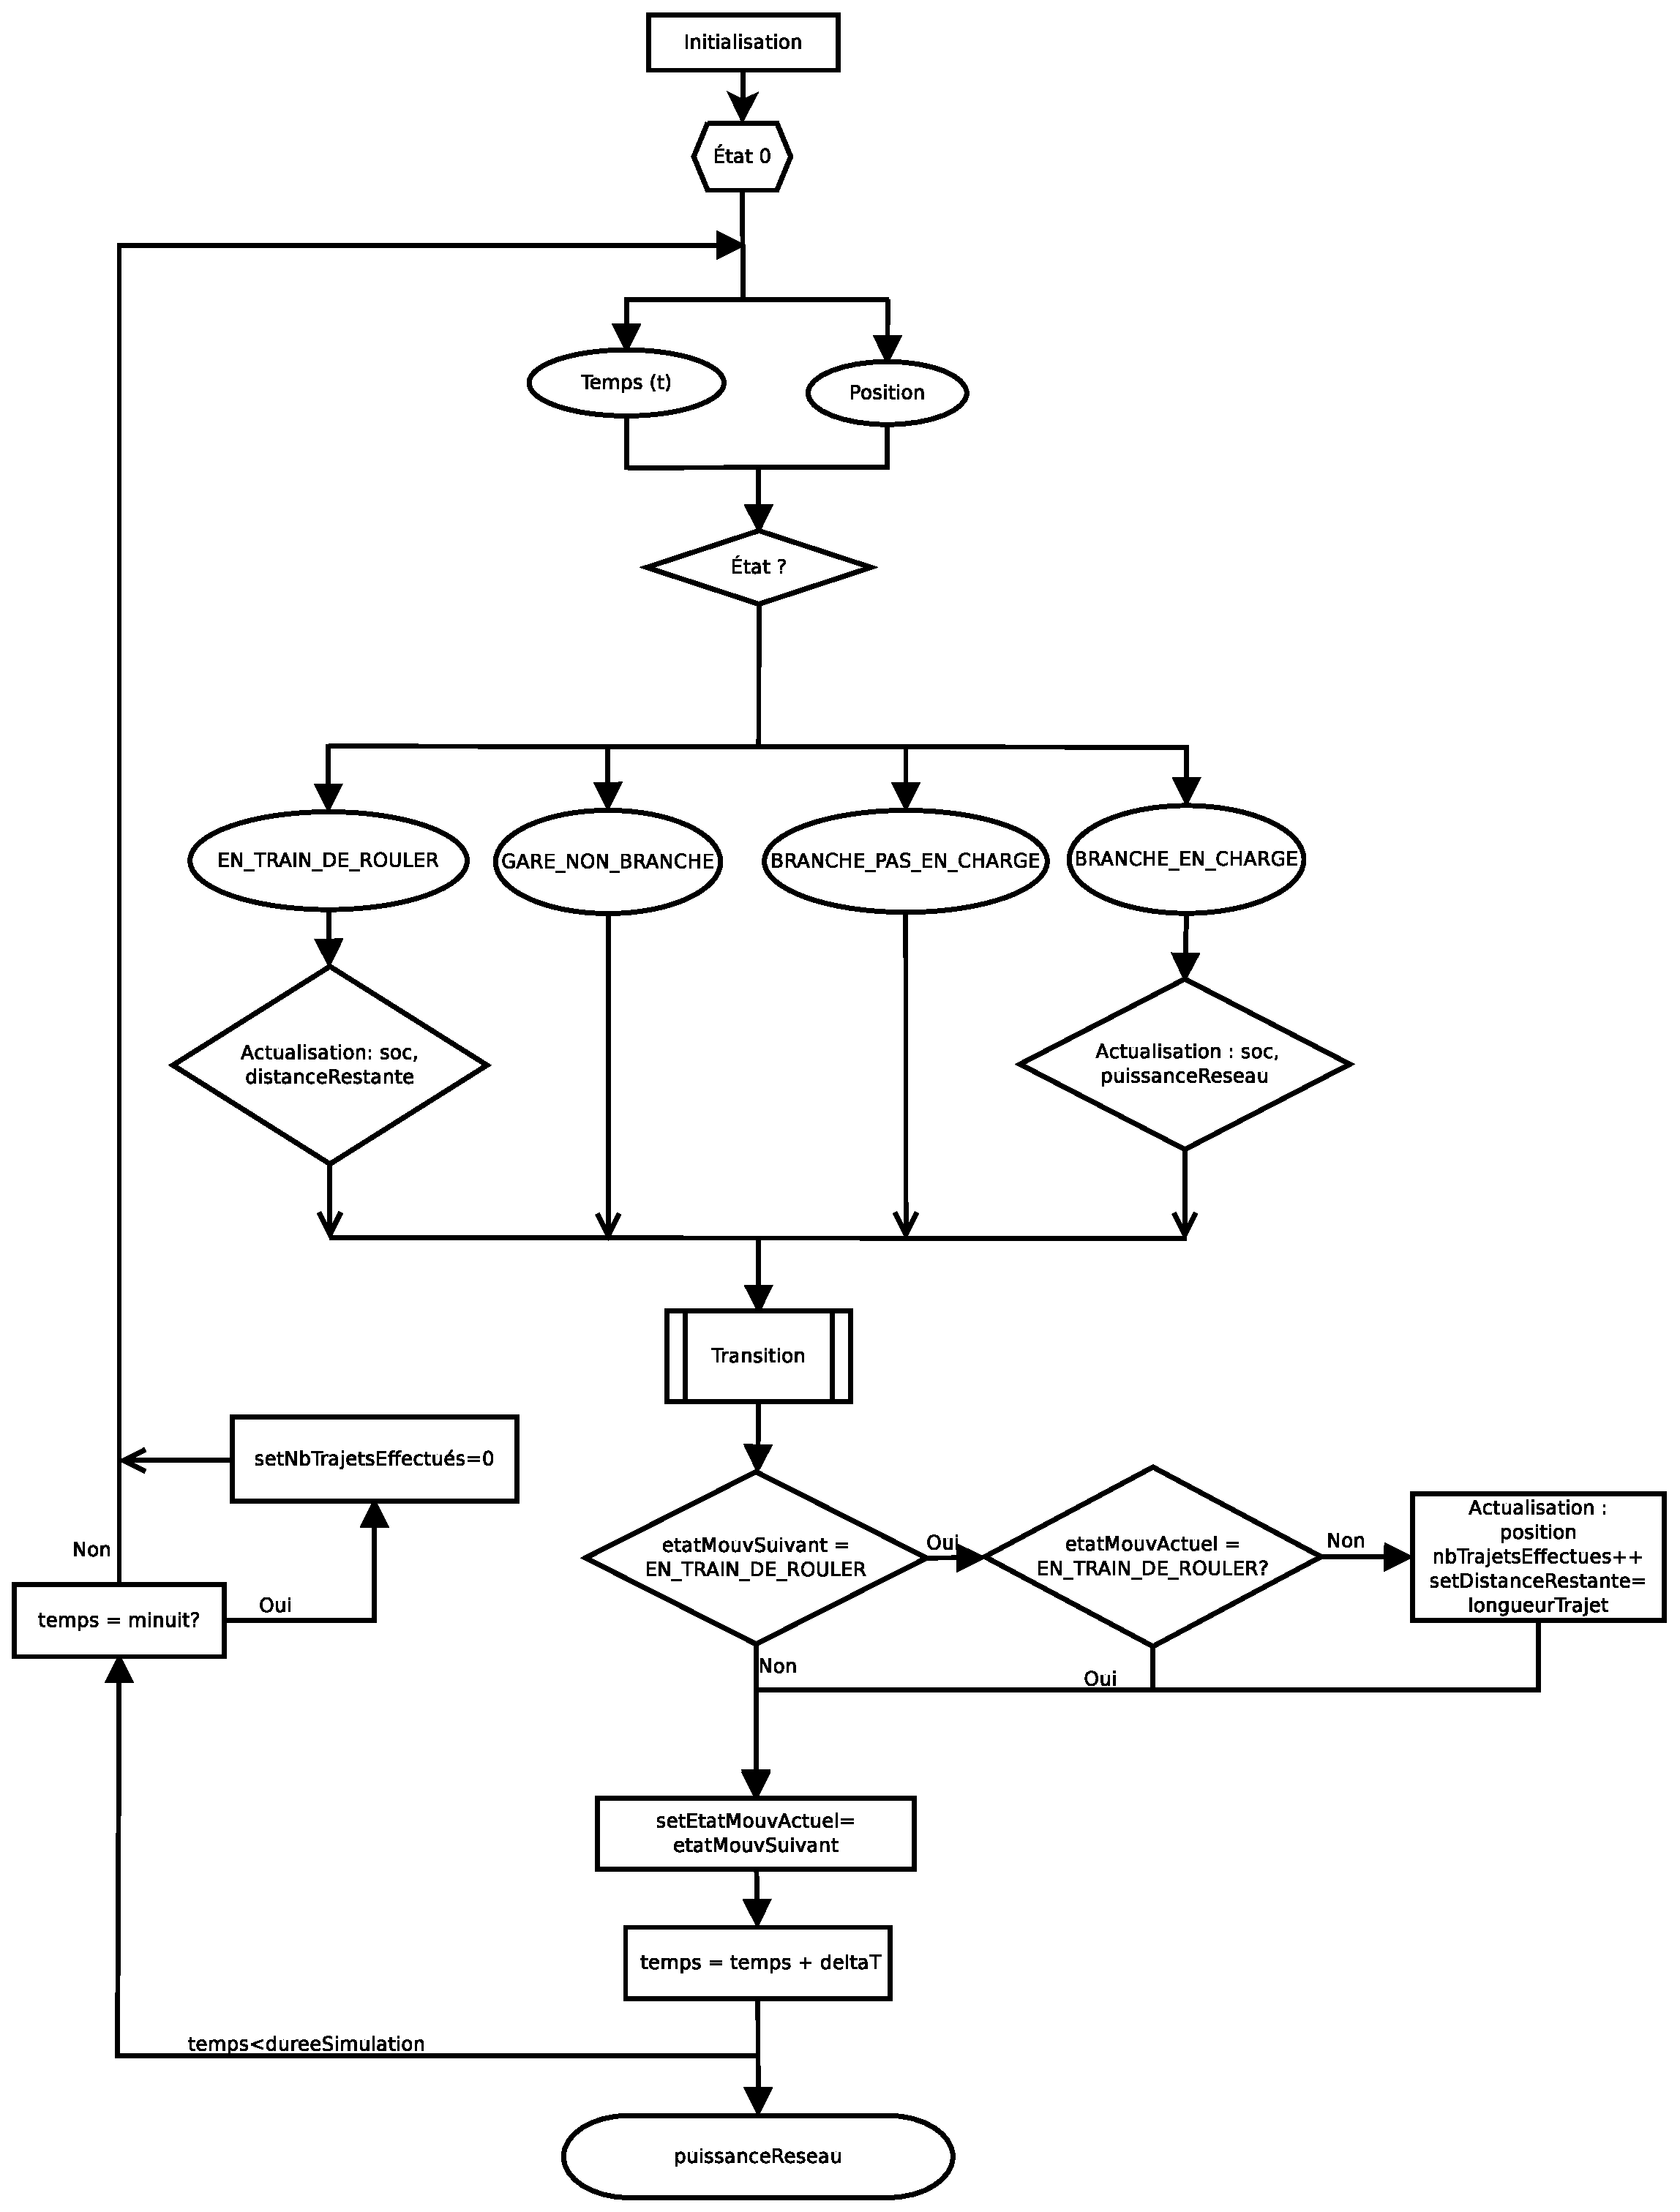
\includegraphics[height=0.9\textheight]{fig/flowPrincipal.eps}
				\caption{Logigramme de la méthode \lstinline{simulation}.\label{fig.flowPrincipal}}
			\end{figure}
			\begin{figure}
				\centering
				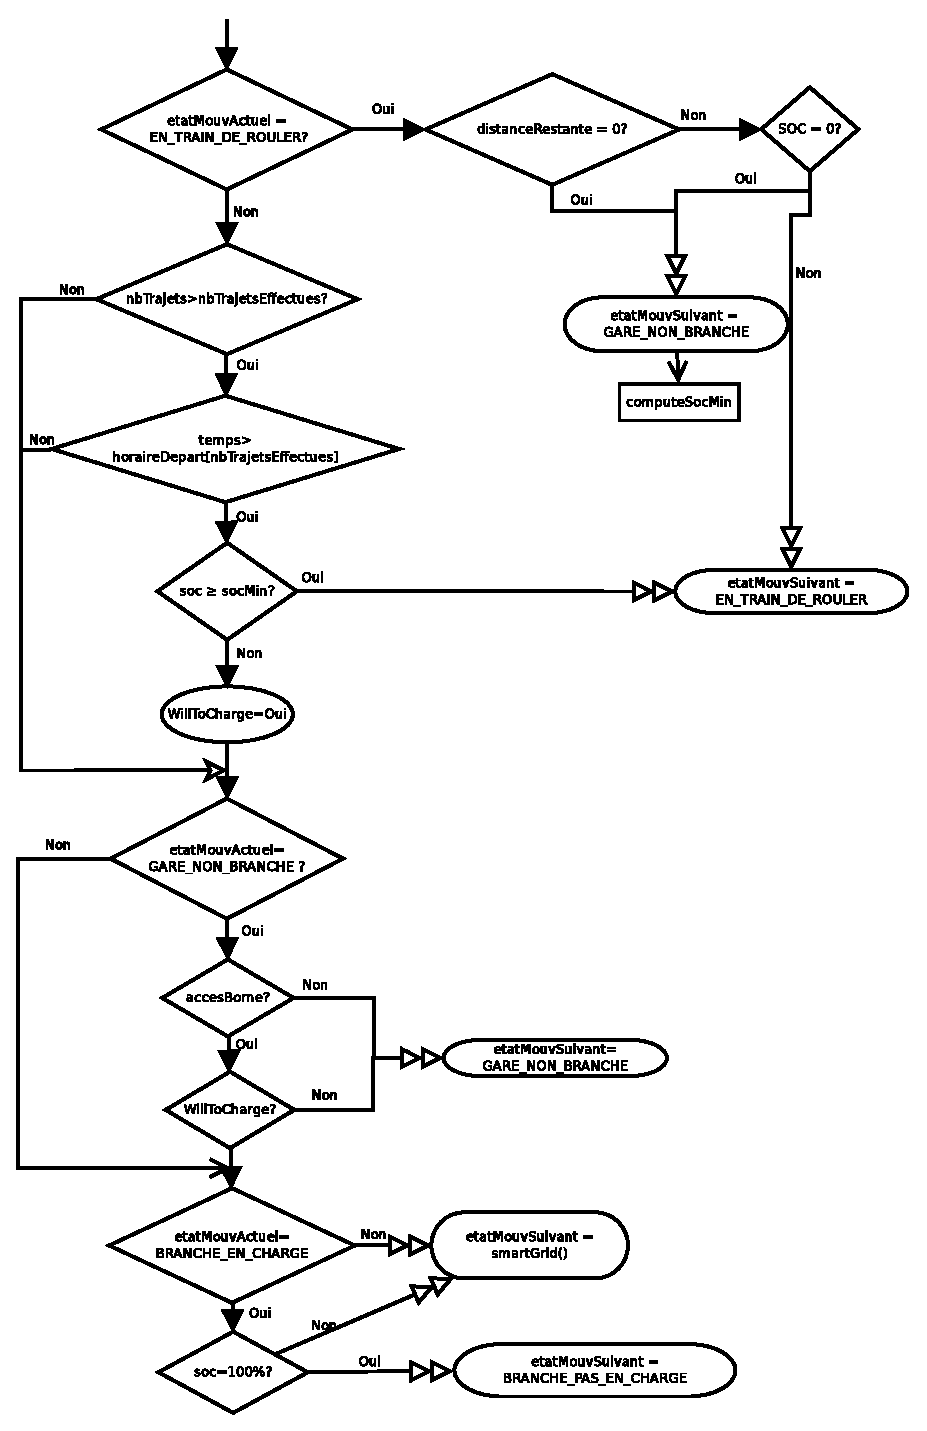
\includegraphics[height=0.9\textheight]{fig/flowTransition.eps}
				\caption{Bloc Transition.\label{fig.flowTransition}}
			\end{figure}
			
			Dans l’organigramme de la méthode \lstinline{transition} on observe deux variables qui n'ont pas encore été décrites.
			
			La première, \lstinline{willToCharge}, est un booléen qui décrit de manière sommaire le comportement de l'utilisateur. On fait l'hypothèse d'un utilisateur rationnel qui ne met son véhicule en charge que lorsque l'autonomie de celui-ci ne lui permet pas de faire les trajets à venir. On simule ainsi le comportement réel des utilisateurs qui, d'après nos données, ne chargent pas leur véhicule de manière systématique, mais en moyenne tous les trois jours.
			
			La deuxième est la fonction 
			\begin{lstlisting}		
    int Vehicule::smartGrid(int temps, int deltaT, 
            int usecase)		
            \end{lstlisting}		
			Cette fonction est définie pour prendre en compte tous les aspects de \smartgrid{}, \emph{Vehicle to Grid}, effacement de charge, etc. C'est dans cette fonction que sont implémentés les différents cas possibles (\emph{use cases}) de monitoring de la charge d'un véhicule. Les \emph{use cases} que nous avons utilisés, et leur implémentation, sont décrits dans la paragraphe~\vref{sec.useCases}. 
			
			D'un point de vue technique, cette fonction retourne un entier qui correspond à un état de charge (\lstinline{BRANCHE_EN_CHARGE} ou \lstinline{BRANCHE_PAS_EN_CHARGE}) selon l'état du véhicule et la méthode d'effacement utilisée, et lève un marqueur qui indique à la suite de la fonction \lstinline|simulation| si le véhicule courant fait du \emph{Vehicle2Grid}. Cette méthode sera le plus souvent imposée par le fournisseur d’électricité dans la réalité.
			
			\bigskip
			
			Lors de l'appel de la fonction \lstinline{main}, la fonction principale du programme, celle-ci prend différents arguments :
			\begin{itemize}
			\item la longueur du pas de temps, $\delta t$ (variable \lstinline{deltaT}), en minutes;
			\item le nombre $D$ de jours correspondant à la durée de la simulation;
			\item le nombre $N$ de véhicules à générer pour la simulation;
			\item le nombre $I$ d'itérations de du programme (on effectue plusieurs fois la même simulation et on moyenne la puissance obtenue).
			\end{itemize}
			
			Le tableau \lstinline{puissanceReseau}, de taille $D \times 1440 / \delta t$ et indexé par les pas de temps de la simulation, est ensuite initialisé. Chaque case contiendra la puissance requise par l'ensemble de la flotte modélisée pour se recharger à l'instant correspondant.
			
			Ensuite la fonction est basiquement une double boucle :
			\begin{enumerate}
			\item une première boucle sur la taille de l'échantillon, qui génère un véhicule par étape et le fait passer dans la deuxième boucle ;
			\item la deuxième boucle est celle décrite dans l'organigramme \vref{fig.flowPrincipal}, indexée par les pas de temps successifs, où à chaque itération la fonction \lstinline{simulation} augmente la valeur la case correspondante de \lstinline{puissanceReseau} d'une unité de puissance ou pas selon que le véhicule est en charge ou non.
			\end{enumerate}
			
			En sortie, on obtient donc un tableau contenant toutes les informations nécessaires au tracé de la courbe de charge imposée par cette flotte au cours du temps.
			
			Après avoir discuté des différents cas de figure que nous avons étudié, c'est cette courbe que nous allons analyser.
			
			%
\begin{tikzpicture}
% style des noeuds
\tikzstyle{etat} = [ellipse, draw]
\tikzstyle{test} = [rectangle, draw]
\tikzstyle{instruct} = [rectangle, draw, rounded corners=4pt]
% style des flèches
\tikzstyle{suite} = [->, >=stealth', thick, rounded corners=4pt]

%% placement des noeuds
\node[instruct] (initialisation) at (0,0) {Initialisation};
\node[etat] (etat0) at (0,-1) {Etat $t$};
\node[test] (whichState) at (0,-2) {etatMouvement ?};
%
%% placement des flèches
\draw[suite] (initialisation) -- (etat0);
\draw[suite] (etat0) -- (whichState);
\end{tikzpicture}
		
		
		\clearpage
		\subsection{  Bornes de recharge et \emph{use case} } \label{sec.useCases}
		
		Nous avons plusieurs possibilités de prédiction en ce qui concerne les infrastructures de recharge. En effet celles-ci peuvent avoir différentes répartitions géographiques sur le territoire (seulement au domicile des utilisateurs ou bien aussi sur leur lieu de travail par exemple).
		De plus il y a aussi différentes possibilités d'implémentation du système \smartgrid{}. Par exemple il peut ne pas y avoir de \smartgrid{} du tout ou bien il peut y avoir un système de \emph{Vehicle to Grid}.
		Nous allons ainsi définir des \textit{use case} (cas d'utilisations) pour les bornes de recharge. 
		
		Nous avons retenu trois scénarios en ce qui concerne la répartition des bornes de recharge :
		\begin{enumerate}
			\item dans la quasi-totalité des cas (\SI{96}{\percent}), une borne au domicile, \SI{33}{\percent} des véhicules possèdent une borne au travail et \SI{14}{\percent} fréquentent des lieux publics où se trouve une borne; cette répartition correspond à la situation actuelle (données statistiques);
			\item les domiciles sont toujours équipés, les entreprises font des efforts et la voie publique s'équipent sur la moitié du territoire;
			\item le véhicule électrique s'est démocratisé : les domiciles sont équipés d'une borne, la majorité des entreprises en proposent à leurs employés et on en trouve sur \SI{90}{\percent} du territoire public.
		\end{enumerate}
		
		\bigskip
		
		On définit aussi différents cas d'utilisation des bornes de recharge en ce qui concerne le \smartgrid{}:
		\begin{enumerate}
			\item pas d'implémentation du \smartgrid{}, on recharge la voiture dès qu'elle est branchée, jusqu'à ce que la batterie soit à sa charge maximale;
			\item on ne recharge pas les voitures pendant les pics de consommation, c'est-à-dire entre 18 heures et 21 heures;
			\item on implémente le système \emph{Vehicle to Grid}, c'est-à-dire qu'entre 18 heures et 21 heures on ne recharge pas mais en plus les véhicules dont l'état de charge est supérieur à \lstinline{socMin} servent à alimenter le réseau en énergie. On considère que c'est l'utilisateur qui rentre ce \lstinline{socMin} dans la borne.  Après 21 heures la recharge normale des véhicules peut reprendre. Nous avons effectué l'hypothèse que ces véhicules en \emph{Vehicle to Grid} fournissent une puissance de \SI{2}{\kilo\watt}. En effet, la rétrocession de l'énergie de la batterie n'atteint pas, avec les technologies actuelles, \SI{100}{\percent}.
		\end{enumerate}
		Notons que tous les usagers de véhicules électriques n'acceptent pas forcément de participer au \smartgrid{} ou encore au \emph{Vehicle to Grid}. On a donc fait l'hypothèse que \SI{75}{\percent} des utilisateurs accepteraient de ne pas recharger leur véhicule durant le pic de consommation et que \SI{66}{\percent} de ces utilisateurs accepteraient de rétrocéder de l'énergie au réseau durant cette période.
		
		\bigskip
		
		Tous ces cas d'utilisations sont volontairement larges et sans nuances afin d'avoir une large fourchette de résultats.
		
		\subsection{Résultats}
			
			\begin{figure}[!h]
				\centering
				\begin{tikzpicture}
					\begin{axis}[
					legend entries = {21/01/2015, 17/07/2014},
					legend style = {at = {(0.95, 0.05)}, anchor = south east}, 
					/pgf/number format/.cd,
					use comma,
					1000 sep={ },
					height = 8cm,
					width = 15cm,
					axis x line = bottom,
					ymin = 0,
					axis y line = left,
				 	xlabel = Heures,
				 	ylabel = Consommation (MW)
				 	]
					\addplot[mark = , smooth, color=blue] table[x=Heures,y=2015-01-21] {fig/courbesRTE.txt};
%					\addlegendentry{21/01/2015};
					\addplot[mark =, smooth, color=red] table[x=Heures,y=2014-07-17] {fig/courbesRTE.txt};
%					\addlegendentry{17/07/2014}
					\end{axis}
				\end{tikzpicture}
				\caption{Courbe de charge du réseau français un jour d'hiver (en bleu) et un jour d'été (en rouge)}
			\end{figure}
			
			\subsubsection{Cas de référence}
			
			Dans l'ensemble de nos modélisations nous avons essayé de partir d'une modélisation de référence et d'en modifier que un ou deux paramètres pour pouvoir comparer aisément les différents résultats obtenus.
			
			Voici les paramètres de ce cas de référence :
			\begin{table}[h!]
			\centering
			\begin{tabular}{|c|c|}
			\hline
			Nombre de Véhicule ($N$) & 163000 \\
			\hline
			\lstinline|deltaT| & \SI{2}{\min} \\
			\hline
			Durée de la simulation & 5 jours \\
			\hline
			Nombre d'itérations & 4 \\
			\hline
			\end{tabular}
			\end{table}
			Le nombre d'itérations correspond au nombre de fois ou nous faisons tourner la boucle de simulation avec $N$ véhicules, et la courbe obtenue est la moyenne des résultats des différentes itérations.
			
			\subsubsection{Influence de l'état de charge initial}
				
				Nous avons tout d'abord étudié l'influence de l'état de charge initial pris en compte dans notre modèle. En effet, il était important de savoir si un choix arbitraire d'état de charge initial influencé grandement ou non nos résultats.
					
				Nous avons donc effectué une première série de modélisation avec les paramètres suivants :
				\begin{table}[h!]
				\centering
				
				\begin{tabular}{|c||c|}
					\hline
					& \lstinline|soc| initial\\
					\hline
					Cas 1 & 100\% \\
					\hline
					Cas 2 & 75\%\\
					\hline
					Cas 3 & 50\%\\
					\hline
					Cas 4 & 25\%\\
					\hline
					Cas 5 & 0\%\\
					\hline
				\end{tabular}
				\end{table}
				Dans ces modélisations, il n'y a aucun \emph{use case} d'utilisé, la fonction \lstinline|smartGrid| retourne la valeur \lstinline|BRANCHE_EN_CHARGE| si la voiture n'est pas pleinement chargé, \lstinline|BRANCHE_PAS_EN_CHARGE| si non.
				
				Les courbes présentées sur la figure \vref{fig.socInitVariable} sont celles obtenues au cinquième jour de modélisation.
				
				\begin{figure}[!h]
					\centering
					\begin{tikzpicture}
						\begin{axis}[
						legend style = {at = {(0.05, 0.95)}, anchor = north west },
						/pgf/number format/.cd,
						use comma,
						1000 sep={ },
						height = 8cm,
						width = 15cm,
						axis x line = bottom,
						axis y line = left,
						xlabel = Heures,
						ylabel = Consommation (kW)
						]
						\addplot[mark = , smooth, color=blue] file{fig/socInitVariables/cas1-100.csv};
						\addlegendentry{Cas 1};
						\addplot[mark = , smooth, color=violet] file{fig/socInitVariables/cas2-075.csv};
						\addlegendentry{Cas 2};
						\addplot[mark = , smooth, color=yellow] file{fig/socInitVariables/cas3-050.csv};
					\addlegendentry{Cas 3};
						\addplot[mark = , smooth, color=cyan] file{fig/socInitVariables/cas4-025.csv};
					\addlegendentry{Cas 4};
						\addplot[mark = , smooth, color=red] file{fig/socInitVariables/cas5-000.csv};
					\addlegendentry{Cas 5};
						\end{axis}
					\end{tikzpicture}
					\caption{Effet de l'état de charge initial sur la courbe de charge résultat au bout de 5 jours. \label{fig.socInitVariable}}
				\end{figure}			
				
				On constate que quelque soit l'état initial choisi il y a convergence des modélisation au bout d'un temps suffisamment long. Cela nous permet de choisir arbitrairement un état de charge initial de \SI{100}{\percent} pour le reste de nos modélisations sans que cette décision n'impacte sur la généralité de notre étude. 
		
				
				\subsubsection{Influence de la répartition des bornes}
				
				Nous avons aussi étudié l'influence de la répartition des bornes sur l'allure de la courbe de charge.
				
				Une fois encore nous avons comparés au cinquième jour de modélisation différents cas : 
				\begin{table}[h!]
				\centering
				\begin{tabular}{|c||c|c|c|}
					\hline
					Nombre de bornes pour 100 véhicules & À la maison & Lieu de travail & Lieu public \\
					\hline
					Cas 1 & 96 & 33 & 14 \\
					\hline
					Cas 2 & 98 & 66 & 50\\
					\hline
					Cas 3 & 99 & 80 & 95\\
					\hline
				\end{tabular}
				\end{table}		
				
				Le cas 1 correspond à la situation actuelle pour les détenteurs de véhicules électriques.
				
				Les courbes sont présentés en figure \vref{fig.repartitionBornes}. Comme dans le cas précédent, aucune implémentation de \smartgrid{} n'est mise en place.
				
				\begin{figure}[!h]
					\centering
					\begin{tikzpicture}
						\begin{axis}[
						legend style = {at = {(0.05, 0.95)}, anchor = north west },
						/pgf/number format/.cd,
						use comma,
						1000 sep={ },
						height = 8cm,
						width = 15cm,
						axis x line = bottom,
						axis y line = left,
						xlabel = Heures,
						ylabel = Consommation (kW)
						]
						\addplot[mark = , smooth, color=blue] file{fig/repartitionBornes/cas1-963314.csv};
						\addlegendentry{Cas 1};
						\addplot[mark = , smooth, color=violet] file{fig/repartitionBornes/cas2-986650.csv};
						\addlegendentry{Cas 2};
						\addplot[mark = , smooth, color=yellow] file{fig/repartitionBornes/cas3-998095.csv};
						\addlegendentry{Cas 3};
						\end{axis}
					\end{tikzpicture}
					\caption{Effet de la répartition des bornes sur la courbe de charge. \label{fig.repartitionBornes}}
				\end{figure}
				
				
				
				\subsubsection{Influence de la mise en place des systèmes \smartgrid{} et \emph{Vehicle to Grid}}
				
				Ici, nous étudions le profil de la courbe de charge lorsque nous implémentons le \smartgrid{} et le \emph{Vehicle to Grid}.
				
				Le cas 1 correspond à notre étude de référence, dans laquelle une flotte de 163000 véhicules est observée sur une durée de 5 jours.
				
				Le cas 2 est la mise en place du \smartgrid{}: on considère que \SI{75}{\percent} des véhicules électriques sont concernés par ce procédé, c'est-à-dire qu'ils acceptent de ne pas se recharger entre \SI{18}{\hour} et $\SI{18}{\hour}+H$ où $H$ est une variable aléatoire uniforme dont la valeur est comprise entre 0 et 3.
				
				Le cas 3 est la mise place du \emph{Vehicle to Grid}: on considère que \SI{66}{\percent} des véhicules électriques qui ont accepté le \smartgrid{} (cas précédent) sont concernés par ce procédé, c'est-à-dire que non seulement ils ne se rechargent pas, mais en plus fournissent une puissance de \SI{2}{\kilo\watt} au réseau électrique, durant la même période que dans le cas précédent.
				
				Les résultats sont présentés sur la figure \vref{fig.usecases}.
				
				\begin{figure}[!h]
					\centering
					\begin{tikzpicture}
						\begin{axis}[
						legend style = {at = {(0.05, 0.05)}, anchor = south west },
						/pgf/number format/.cd,
						use comma,
						1000 sep={ },
						height = 8cm,
						width = 15cm,
						axis x line = bottom,
						axis y line = left,
						xlabel = Heures,
						ylabel = Consommation (kW)
						]
						\addplot[mark = , smooth, color=blue] file{fig/useCases/cas1.csv};
						\addlegendentry{Cas 1};
						\addplot[mark = , smooth, color=violet] file{fig/useCases/cas2.csv};
						\addlegendentry{Cas 2};
						\addplot[mark = , smooth, color=yellow] file{fig/useCases/cas3.csv};
						\addlegendentry{Cas 3};
						\end{axis}
					\end{tikzpicture}
					\caption{Effet de la mise en place des systèmes \smartgrid{} et \emph{Vehicle to Grid} sur la courbe de charge. \label{fig.usecases}}
				\end{figure}

		


\section*{Conclusion}

\bibliographystyle{ieeetr-fr}
\bibliography{parts/sources}

\end{document}
